\documentclass{acm_proc_article-sp}
\usepackage{amsmath}

\begin{document}

\title{A Search System for Tree-Structrued \\ Mathematical Formula in {\ttlit LaTeX} Format}

\numberofauthors{2} 
\author{
\alignauthor Wei Zhong,\; Hui Fang\\
       \affaddr{Dept. of Electrical and Computer Engineering}\\
       \affaddr{University of Delaware}\\
       \affaddr{Newark, DE USA}\\
       \email{\{zhongwei, hfang\}@udel.edu}
}

\maketitle
\begin{abstract}
The special characteristic of mathematical language, compared with normal text content, makes mainstream retrieval models (e.g. ``bag of words'' model) deficient to provide good result in cases where query is in mathematical language. In this paper, we address the difficulties of similarity identification of mathematical contents and present a search system specifically for mathematical contents, more precisely, a system to tokenize mathematical content in \LaTeX{} into formulas, to transform a tree-structured formula to what we call ``branch words'', and to score the relevance degree between ``branch words''. Using this system, we show the potential and possibility to tackle the problems in mathematical searching.
\end{abstract}

\category{H.3}{Information Search and Retrieval}{Miscellaneous}
\terms{Algorithms}

\keywords{mathematical searching, language processing, search engine}

\section{Introduction}
Unlike normal text content, mathematical language, by its nature, has many differences from normal text content. First, one mathematical formula may use different notations and thus has different representations.\footnote{An example, $a^2 + b^2 = c^2$ can be described as $x^2 + y^2 = z^2$ as well.} Second, two semantically different mathematical document can contain the same number of terms.\footnote{Consider $ax+(b+c)$ and $(a+b)x+c$.} Also, the order of terms in math language sometimes matters but can be mutable in other cases, which implies it is impractical to uniformly apply one single language model to mathematical content.

Currently existing and working mathematical searching systems that we can find online, primarily are \textit{WolfraAlpha}\footnote{http://www.wolframalpha.com/}, \textit{(uni)quation}\footnote{http://uniquation.com/} and \textit{MWS}\footnote{http://search.mathweb.org/}. \textit{WolfraAlpha} mainly focus on computation and evaluation of mathematical equation input rather than searching the similar equation. \textit{(uni)quation} is able to solve the problems addressed above in this section but it is not under development and the approach it uses to handle math content is currently unclear.\footnote{http://rystsov.info/2009/05/01/uniquation.html} \textit{WMS} uses \textit{term indexing}\cite{McCune, Stickel} which we are not using here, to discriminate mathematical structures.

Our system tries a different approach to make use of the structure of mathematical formula to solve the problems addressed above. It uses an efficient way to parse and tokenize mathematic formula, to transform a tree-structured formula to a more comparable structure, and is able to score and rank results.

\section{System Description}
The system presented by us has a WEB front-end to accept user input in \LaTeX{} format and pass it to the back-end. The back-end, mainly consists of a parser and a search program. The function of parser is to do tokenization and tree construction as well as storing output structure into our collection. The search program compares the query and document and evaluates the similarity of them, gives the final ranking through output file for the WEB front-end \texttt{CGI program} (Apache Common Gateway Interface, we use it as a way to interact between WEB interface and back-end program) to read. We input mathematical content in \LaTeX{} as document to our parser by either manually creating or by a crawler script specifically targeting at mathematical content website \textit{Mathematics Stack Exchange}\footnote{http://math.stackexchange.com/}.

\subsection{Tokenization and Tree Construction}
The parser is designed to tokenize a subset of mathematic related \LaTeX{} language, we utilize \texttt{Lex/Yacc} tools to tokenize the LaTex Language and construct a ``tree'' for each equation. The LALR parser generator of \texttt{Yacc} can handle language efficiently in guaranteed linear time\cite{Knuth}. The grammar we use will parse mathematical content into different classes of tokens including variables, different basic math operators, equal class, times class, fraction class and square root. And we choose to omit undefined control sequence for the sake of robustness. 

When a grammar is reduced, the tokens is converted to a tree node directly or by attaching sub-trees which is reduced previously to the new root. In this way, we will finally get a tree structured representation.

\begin{figure}
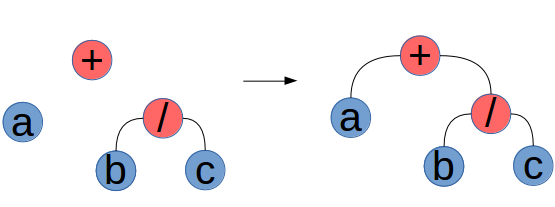
\epsfig{file=attach.png, height=1.2in, width=3in}
\caption{Example of Sub-tree generation for the addition grammar.}
\end{figure}

Some operations may have commutative property, in these cases\footnote{In our system, the cases where we apply commutative property include \textit{addition} and \textit{multiplication} operations.}, all the sons in two adjacent levels will be attached to the same root.

\begin{figure}
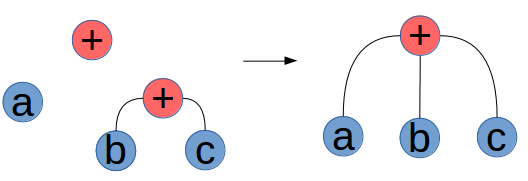
\epsfig{file=case.png, height=1in, width=3in}
\caption{Cases where commutative property applies.}
\end{figure}

\subsection{Extraction of Branch words}
After constructing a tree, A ``branch word'' is extracted by taking tokens from the leaves to the root of a tree in order. Branch words are used to be compared with those of other trees. 

\begin{figure}
\centering
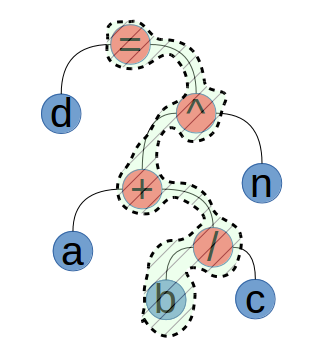
\epsfig{file=branch.png, height=1.9in, width=1.8in}
\caption{Illustration of One Branch Word for formula $(a+\frac{b}{c})^n = d$.}
\end{figure}

We notice that one math equation can use different symbol sets, so we choose not to distinguish the leaves' actual symbol in the branch word. We also notice the branch word is not enough to distinguish trees, an example would be the two equations $(a + b + c)\times (d + e)$ and $(a + b) \times (c + d + e)$, they have the same branch words yet have different semantic meaning in mathematical language. To avoid this flaw we further introduce the weight for any node $n_i$ in a branch word, defined by the sum of that of its successors, which is given by:
$$
w(n_i) = \sum\limits_{n} \; 1 \;, \qquad n \in \left\{n_i \cup succ(n_i) \right\}
$$

\subsection{Indexing and Storage}
The storage of mathematical formulas in our system, contains all the branch words from each tree as well as the weight information of each node in branch words. To enable efficient retrieval, branch words are stored in file system where the path is named by token names of a branch word (with weight information) in order\footnote{One example can be \texttt{./collection/var/frac/add}}. The path where a branch word resides also stores a ``posting'' file recording all the documents in the collection which contain that branch word.

\subsection{Comparing and Scoring}
In our system, comparing two pieces of mathematical content is essentially to compare all the branch words from one content with those of the other, calculate the similarity degree between two branch words. In order to rank-order the documents matching a query, a score with respect to the query for each matching document is computed by sum the similarity degree for each related document in all the collection, then the system ranks all the related documents using the sum score.

For the detailed caculation, we put some notations here: Let $m$ be the number of continuous weight matches between two branches from the beginning of the branch word. For one branch word $b$, let $n_b$ be the number of same branch words from document that extracts $b$, $\  l_b$ be the length of branch word $b$. Then for branch word $i$ in query and branch word $j$ in related document $k$. The formulas we use to calculate both relevance $R$ between two branch words and the score $S_k$ for document $k$ are:
\begin{figure*}
\centering
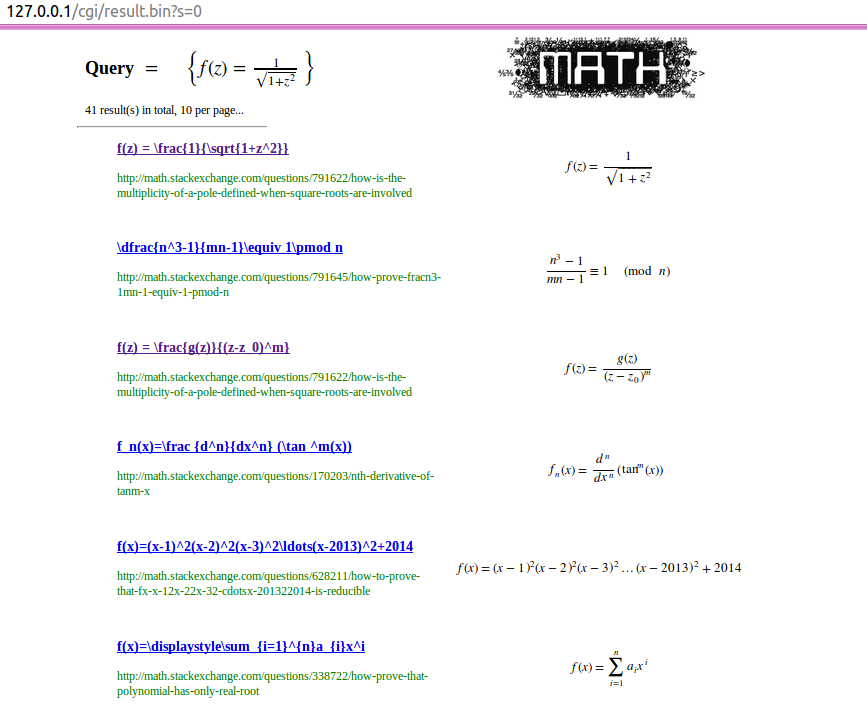
\epsfig{file=screen.png, height=3.8in, width=4.7in}
\caption{WEB interface for Our Prototype System}
\end{figure*}

\begin{align}
\label{shi}
R_{i,j} &= \alpha \cdot \min(n_i, n_j) \cdot \frac{m}{l_i} + \frac{1}{\lvert n_i - n_j \rvert + 1} \cdot \frac{m}{\max(l_i, l_j)} \\
S_k &= \sum_{i}\sum_{j}\,R_{i,j}
\end{align}
Where $\alpha$ is a large constant number to prioritize the first term in \eqref{shi}.

\subsection{WEB front-end}
The WEB interface contains a homepage for user to input query in an input box, just like a normal search engine does. The difference is, our interface accepts \LaTeX{} as input and has a render preview for math equations. The WEB interface uses CGI program as a middle layer to both get user query (using \textit{libcurl} library to unescape the URL encoding) and generate ranking page in HTML (by writing to the standard output) from the output file written by back-end program.

\section{Future Work}
Our current system does not distinguish variables and constant tokens from each other. Although this is good in cases $a^2 + b^2$ and $x^2 + y^2$ is treated as the same, but it is obviously not reasonable to let $n+\frac{1}{n}$ equal with $a+\frac{1}{b}$. Future work may involve unification algorithm\cite{Baader} to better evaluate the relevance between formula symbols. Second, the resulting collection with input data from our crawler is not as good as that with the input data we manually choose. Part of the issue arises due to the ambiguity of high-level spaces\cite{Richard}. Erroneous tight-binding spaces and failure in interpretation will result in blank token in our system, which may be deduced by our parser as \textit{multiplication} operation. Moreover, statistical evaluation needs to be done on the effectiveness of our search results. But above all, the most important goal of future work is to explore the unrevealed potential of its usefulness.

\section{Conclusions}
In this paper, we introduce and present an experimental mathematical formula search system, also demonstrate the possibility of our approach which tries to utilize the structure of math formula to provide better search result for mathematical content. 

Our prototype system is able to return relevant result in cases where the query uses a different set of symbol notations from the document, and a change-of-order for symbols that has mutable property. While there is a lot of future work ahead, the rich possibilities and huge potential for math-aware searching remain inspiring to us.

\bibliographystyle{unsrt}
\bibliography{sigproc}  % sigproc.bib is the name of the Bibliography in this case

\end{document}
